\documentclass[11pt]{article}

\usepackage[margin=0.78in]{geometry}
\usepackage[T1]{fontenc}
\usepackage{lmodern}
\usepackage{microtype}
\usepackage{graphicx}
\usepackage{amsmath}
\usepackage{booktabs}
\usepackage{tabularx}
\usepackage{array}
\usepackage{xcolor}
\usepackage{tikz}
\usepackage{enumitem}
\usepackage{placeins}
\usepackage{hyperref}
\usetikzlibrary{arrows.meta,positioning}

\definecolor{linegray}{RGB}{100,106,112}
\definecolor{lightblue}{RGB}{231,238,247}
\definecolor{lightgreen}{RGB}{229,241,235}
\definecolor{lightorange}{RGB}{249,237,221}
\definecolor{lightred}{RGB}{247,231,229}
\definecolor{blue}{RGB}{49,90,138}

\hypersetup{
  colorlinks=true,
  linkcolor=blue,
  urlcolor=blue,
  pdftitle={OCR Error Recovery in Egyptian Medicine Search}
}

\graphicspath{{../results/04_model_predictions/figures/}}
\newcolumntype{Y}{>{\raggedright\arraybackslash}X}
\newcommand{\code}[1]{\texttt{#1}}
\newcommand{\chart}[1]{%
  \includegraphics[width=0.96\linewidth,height=0.70\textheight,keepaspectratio]{#1.pdf}}
\newenvironment{figureinsights}{%
  \par\smallskip\begin{minipage}{0.94\linewidth}\small
  \textbf{Insights}\begin{enumerate}[leftmargin=1.5em,itemsep=1pt,topsep=2pt,parsep=0pt]
}{%
  \end{enumerate}\end{minipage}
}

\setlength{\parindent}{0pt}
\setlength{\parskip}{0.42em}
\renewcommand{\arraystretch}{1.12}
\clubpenalty=10000
\widowpenalty=10000
\displaywidowpenalty=10000

\title{\textbf{OCR Error Recovery in Egyptian Medicine Search}\\
\large What was tested, what failed, and why}
\author{medicine-search-clean engineering analysis}
\date{19 July 2026}

\begin{document}
\maketitle

\begin{abstract}
This report tests whether Algorithm 4, the medicine-family search system, can recover an Egyptian medicine family
from text already produced by an OCR model. The input is an OCR string, not a
prescription image. Across all 595 observations, Algorithm 4 reaches 50.25\%
Hit@1 (verified family ranked first) and 73.78\% Hit@20 (verified family within
the first 20). The primary denominator, which is the score to cite, removes 17
queries that exactly name a different real drug and gives each distinct
query-target pair one vote; its 464 cases reach 47.63\% Hit@1 and 71.12\%
Hit@20. An extreme prediction has compact Levenshtein distance, calculated
after removing spaces and punctuation, divided by target length above 0.60.
All 121 extreme predictions remain in the inclusive 595-row diagnostic view.
Compact distance four or more creates 140 of its 156 top-20 misses.
\end{abstract}

\section{What Was Tested}

The experiment starts after OCR. Fourteen OCR models had already read medicine
images and written their text predictions to \code{predictions.csv}. Algorithm 4
receives one prediction at a time. The verified family is hidden until scoring.

\begin{figure}[htbp]
\centering
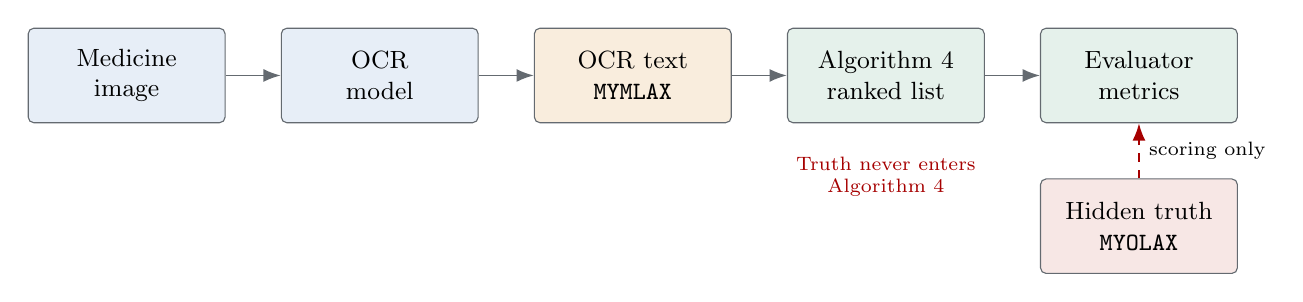
\begin{tikzpicture}[
  node distance=7mm,
  block/.style={rectangle,rounded corners=2pt,draw=linegray,align=center,
                minimum width=25mm,minimum height=12mm,font=\small},
  arrow/.style={-{Latex[length=2.2mm]},draw=linegray,line width=0.6pt},
  hidden/.style={-{Latex[length=2.2mm]},draw=red!65!black,dashed,line width=0.7pt}
]
\node[block,fill=lightblue] (image) {Medicine\\image};
\node[block,fill=lightblue,right=of image] (ocr) {OCR\\model};
\node[block,fill=lightorange,right=of ocr] (text) {OCR text\\\code{MYMLAX}};
\node[block,fill=lightgreen,right=of text] (search) {Algorithm 4\\ranked list};
\node[block,fill=lightgreen,right=of search] (score) {Evaluator\\metrics};
\node[block,fill=lightred,below=of score] (truth) {Hidden truth\\\code{MYOLAX}};
\draw[arrow] (image) -- (ocr);
\draw[arrow] (ocr) -- (text);
\draw[arrow] (text) -- (search);
\draw[arrow] (search) -- (score);
\draw[hidden] (truth) -- node[right,font=\scriptsize]{scoring only} (score);
\node[font=\scriptsize,text=red!65!black,below=3mm of search,align=center]
  {Truth never enters\\Algorithm 4};
\end{tikzpicture}
\caption{Read left to right: the OCR output \code{MYMLAX} enters Algorithm 4,
while hidden truth \code{MYOLAX} reaches only the evaluator. The benchmark
therefore measures medicine-search recovery after OCR; it does not rerun OCR or
evaluate prescription segmentation.}
\label{fig:pipeline}
\begin{figureinsights}
  \item The benchmark isolates search recovery from OCR recognition quality.
  \item Keeping the verified target outside Algorithm 4 prevents answer leakage during retrieval.
\end{figureinsights}
\end{figure}

\begin{table}[htbp]
\centering
\small
\begin{tabularx}{\linewidth}{@{}p{0.13\linewidth}p{0.30\linewidth}Y@{}}
\toprule
\textbf{Stage} & \textbf{Concrete example} & \textbf{Meaning} \\
\midrule
Input & \code{MYMLAX}, model = EasyOCR & Text delivered to Algorithm 4. \\
Process & Search 25,066 catalog medicines & Generate and rank family candidates. \\
Output & \code{MYOLAX} at rank 1 & The verified family is recovered first. \\
Scoring & H@1 = 1, H@20 = 1 & The evaluator compares output with hidden truth. \\
\bottomrule
\end{tabularx}
\caption{The example traces one row from OCR input \code{MYMLAX} through a
25,066-medicine search to \code{MYOLAX} at rank 1. The expected family affects
metrics, never retrieval.}
\label{tab:contract}
\end{table}

The 595 rows are OCR \emph{observations}, not necessarily 595 unique images.
Several models can produce predictions for the same medicine. The report has
477 unique normalized query-target pairs and 118 repeated observations.

\FloatBarrier
These repeated rows change which denominator answers which question. The next
section fixes the counting rules before any aggregate score is interpreted.
\section{Data Contract and Definitions}

An \textbf{observation} is one OCR model output paired with one verified
medicine target. For example, EasyOCR output \code{MYMLAX} paired with verified
target \code{MYOLAX} is one observation. Another model producing the same pair
is another observation, but not another unique query-target pair.

\begin{table}[htbp]
\centering
\small
\begin{tabularx}{\linewidth}{@{}>{\raggedright\arraybackslash}p{0.29\linewidth}rY@{}}
\toprule
\textbf{Dataset object} & \textbf{Size} & \textbf{Meaning} \\
\midrule
Source prediction CSV & 595 rows $\times$ 15 columns & OCR text, verified target, OCR model, lengths, source alignment counts, normalized distances, and operation sequence. No source cell is missing. \\
Algorithm result CSV & 595 rows $\times$ 44 columns & One joined search result per source row, including candidates, ranks, Hit@k, cohort, split, decision, and latency. \\
OCR source models & 14 & Models contribute 26--73 rows each; the mean is 42.5 rows per model. \\
Verified target families & 27 & Targets contribute 1--92 rows each; the mean is 22.04 rows per target. \\
Unique raw OCR strings & 481 & Repeated strings remain separate observations. Mean repetition is 1.24 rows per raw string. \\
Unique compact query-target pairs & 477 & Spaces, punctuation, and case are removed before duplicate pairs are identified. \\
Scored observations & 578 & The 17 real-drug collisions remain diagnostic rows but do not enter the primary correctness denominator. \\
Primary scored unique pairs & 464 & Each scored compact query-target pair receives one vote. This is the primary benchmark denominator. \\
\bottomrule
\end{tabularx}
\caption{The two CSV files join one-to-one. ``Row count'', ``unique-pair count'',
and ``scored count'' are different denominators and therefore produce different
accuracy values.}
\label{tab:data-contract}
\end{table}

\begin{center}
\fcolorbox{linegray}{lightblue}{%
\begin{minipage}{0.92\linewidth}
\textbf{Which number should you report?} Cite the primary 464-pair result,
47.63\% Hit@1 and 71.12\% Hit@20, when comparing search algorithms because each
distinct scored query-target pair receives one vote. Use the inclusive 595-row
result, 50.25\% Hit@1 and 73.78\% Hit@20, when auditing every supplied OCR
observation, including repetitions and real-drug collisions.
\end{minipage}}
\end{center}

The \textbf{compact form} lowercases text and removes spaces, punctuation, and
other non-alphanumeric characters. Thus \code{CLEX A NE} and \code{CLEXANE}
share the compact form \code{clexane}. Let $q_c$ be the compact OCR query and
$y_c$ the compact verified target. The search-side distance and normalized
distance are
\[
d=L(q_c,y_c), \qquad r=\frac{d}{\max(|y_c|,1)},
\]
where $L$ is Levenshtein distance. One insertion, deletion, or replacement costs
one. A row is \textbf{extreme} when $r>0.60$, unless the query exactly names a
different catalog family, which takes priority as a real-drug collision.
For \code{GHONT} $\rightarrow$ \code{CALAMINE}, $d=7$, $|y_c|=8$, and
$r=7/8=0.875$; the row is extreme.

The $0.40$ and $0.60$ boundaries are fixed operational review bands inherited
from the benchmark methodology. They were not fitted to Algorithm 4 results and
do not represent clinical risk probabilities. The original filtering policy
sent $r>0.60$ rows to manual review. This analysis keeps those rows and reports
their performance instead of rejecting them.

The source CSV also supplies a character alignment that can retain spaces. Its
\code{edit\_distance\_count} can therefore differ slightly from compact distance
$d$. Figures explicitly say \emph{source distance} or \emph{compact distance};
the terms are not interchangeable.

\begin{table}[htbp]
\centering
\small
\begin{tabular}{@{}llllr@{}}
\toprule
\textbf{Representation} & \textbf{OCR text} & \textbf{Target} & \textbf{Calculation} & \textbf{Result} \\
\midrule
Source alignment & \code{CLEX A NE} & \code{CLEXANE} & two retained spaces & $d_s=2$, $2/7=0.286$ \\
Compact search & \code{clexane} & \code{clexane} & spaces removed first & $d=0$, $r=0$ \\
\bottomrule
\end{tabular}
\caption{One OCR pair can have nonzero source distance but zero compact distance.
Source plots describe the supplied alignment; search cohorts use compact $d$ and $r$.}
\label{tab:distance-example}
\end{table}

\begin{table}[htbp]
\centering
\small
\begin{tabularx}{\linewidth}{@{}p{0.16\linewidth}Y@{}}
\toprule
\textbf{Term} & \textbf{Definition used in this report} \\
\midrule
$n$ & Number of rows in the displayed group. It is the denominator for a group percentage. \\
Mean & Sum of values divided by $n$. Large outliers can move it. \\
Median & Middle value after sorting. Half the rows are below it and half are above it. \\
Q1--Q3 & Middle 50\% of rows, from the 25th to the 75th percentile. \\
Hit@k & Percentage of rows whose verified family appears at rank $k$ or earlier. \\
Failure rate & Top-20 misses in a group divided by rows in that group. \\
Failure share & Top-20 misses in a group divided by all top-20 misses. \\
\bottomrule
\end{tabularx}
\caption{Every average, rate, and percentage in later figures uses one of these
definitions. Group plots print $n$ beside the group name.}
\label{tab:stat-definitions}
\end{table}

\begin{figure}[htbp]
\centering\chart{00_dataset_overview}
\caption{Panels A and B count observations by target-family split and cohort;
panel C counts observations at each source edit distance; panel D partitions
Algorithm 4 outcomes. The CSV is dominated by standard OCR errors, but extreme
predictions form one fifth of all rows and most are outside the top 20. Cohort
examples are standard
\code{ABISAGLOR}$\rightarrow$\code{ABASAGLAR}, high-distance
\code{OSMOL}$\rightarrow$\code{OSTOCAL}, extreme
\code{GHONT}$\rightarrow$\code{CALAMINE}, fragment
\code{RIVOTRI}$\rightarrow$\code{RIVOTRIL}, collision
\code{RIVOTRIL}$\rightarrow$\code{RIVO}, and compact exact
\code{TO CO}$\rightarrow$\code{TOCO}. In panel C, mean 3.03 exceeds median 2
because a small severe tail pulls the mean upward.}
\label{fig:00}
\begin{figureinsights}
  \item The 20.2\% family-disjoint holdout provides a genuine unseen-family check rather than a random-row split.
  \item High and extreme corruption together cover 36.4\% of the CSV, so mild typo performance cannot dominate the benchmark.
  \item Mean source distance exceeds the median because a small severe tail changes the aggregate.
  \item The 140 ranking failures and 156 retrieval failures require different algorithm changes.
\end{figureinsights}
\end{figure}

\begin{table}[htbp]
\centering
\small
\begin{tabular}{@{}lrrrrr@{}}
\toprule
\textbf{Numeric field} & \textbf{Mean} & \textbf{Median} & \textbf{Q1} & \textbf{Q3} & \textbf{Min--max} \\
\midrule
OCR-output length (characters) & 7.24 & 7.00 & 6.00 & 9.00 & 1--13 \\
Verified-target length (characters) & 7.27 & 8.00 & 6.00 & 9.00 & 4--9 \\
Source edit distance (operations) & 3.03 & 2.00 & 1.00 & 4.00 & 1--10 \\
Source distance / target length & 0.434 & 0.333 & 0.200 & 0.556 & 0.111--2.000 \\
Compact edit distance (operations) & 2.96 & 2.00 & 1.00 & 4.00 & 0--10 \\
Compact distance / target length & 0.425 & 0.333 & 0.200 & 0.556 & 0.000--2.000 \\
Source similarity & 0.566 & 0.667 & 0.444 & 0.800 & $-1.000$--0.889 \\
Returned candidate count & 28.66 & 31.00 & 25.00 & 34.00 & 0--44 \\
Query latency (ms) & 15.30 & 14.27 & 10.45 & 18.88 & 0.04--39.83 \\
\bottomrule
\end{tabular}
\caption{Global descriptive statistics over all 595 observations. A normalized
distance can exceed 1 when the number of edits exceeds the target length;
similarity then becomes negative.}
\label{tab:descriptive-stats}
\end{table}

Target-family hashing keeps KETOROLAC's 92 rows in development for analysis and
tuning, and VIGOREX's 32 rows in holdout for unseen-family checking. Other label
examples are SAFE/one-edit \code{KETONOLAC}$\rightarrow$\code{KETOROLAC},
two-edit \code{ABISAGLOR}$\rightarrow$\code{ABASAGLAR}, multi-edit
\code{ABASCOLOGY}$\rightarrow$\code{ABASAGLAR}, visible-fragment
\code{RIVOTRI}$\rightarrow$\code{RIVOTRIL}, CAUTION/high-distance
\code{OSMOL}$\rightarrow$\code{OSTOCAL}, and DANGEROUS/collision
\code{RIVOTRIL}$\rightarrow$\code{RIVO}. An ambiguous
\code{ABISAGLOR}$\rightarrow$\code{ABASAGLAR} response lists candidates;
no-match \code{H}$\rightarrow$\code{RIVO} returns zero. Decision examples are
possible \code{KETONOLAC}, equal-distance
\code{OSTEOCL}$\rightarrow$\code{OSTOCAL}, and family-variant
\code{ABISAGLOR}.

\begin{table}[htbp]
\centering
\small
\begin{tabularx}{\linewidth}{@{}p{0.17\linewidth}p{0.43\linewidth}Y@{}}
\toprule
\textbf{Categorical field} & \textbf{Complete distribution} & \textbf{Assignment rule} \\
\midrule
Split & Development 475; holdout 120 & Deterministic hash of target family; one target cannot cross splits. \\
Danger & SAFE 342; CAUTION 236; DANGEROUS 17 & DANGEROUS for real-drug collision; CAUTION for compact query length $\leq4$ or $r>0.40$; SAFE otherwise. \\
Mistake type & 1 edit 172; 2--3 edits 217; multi-edit 172; real-drug collision 17; prefix/suffix fragment 17 & Collision and fragment rules first; otherwise compact edit count. \\
Response status & Ambiguous 583; no match 12 & Ambiguous returns candidates without certifying one; no match returns zero candidates. \\
Decision type & Possible matches 330; equal-distance ambiguity 155; family-variant selection 98; no match 12 & Algorithm 4 response branch after candidate generation and family grouping. \\
Search outcome & Rank 1 success 299; ranks 2--20 success 140; outside top 20 156 & Position of the verified family in the returned family ranking. \\
\bottomrule
\end{tabularx}
\caption{Complete distributions for the major categorical columns used in the
paper. Counts in each row sum to 595. Cohort counts appear separately in
Table~\ref{tab:cohort-rules}. Mistake type describes the compact edit pattern;
cohort applies severity and collision priority, so their fragment counts need
not match.}
\label{tab:categorical-distributions}
\end{table}

\FloatBarrier
The contract now fixes every denominator and label; the next section follows one
OCR row through retrieval and scoring so those definitions become concrete.
\section{One Complete Example}

EasyOCR produced \code{MYMLAX}; the verified family is \code{MYOLAX}. Five
characters match and one character is substituted. Algorithm 4 returns 36
candidates and places \code{MYOLAX} first.

\begin{figure}[htbp]
\centering
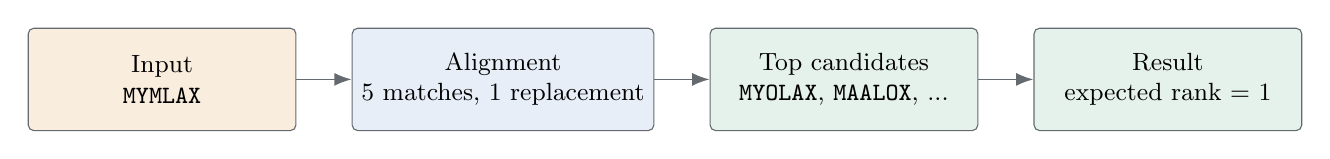
\begin{tikzpicture}[
  node distance=7mm,
  block/.style={rectangle,rounded corners=2pt,draw=linegray,align=center,
                minimum width=34mm,minimum height=13mm,font=\small},
  arrow/.style={-{Latex[length=2.2mm]},draw=linegray,line width=0.6pt}
]
\node[block,fill=lightorange] (a) {Input\\\code{MYMLAX}};
\node[block,fill=lightblue,right=of a] (b) {Alignment\\5 matches, 1 replacement};
\node[block,fill=lightgreen,right=of b] (c) {Top candidates\\\code{MYOLAX}, \code{MAALOX}, ...};
\node[block,fill=lightgreen,right=of c] (d) {Result\\expected rank = 1};
\draw[arrow] (a) -- (b);
\draw[arrow] (b) -- (c);
\draw[arrow] (c) -- (d);
\end{tikzpicture}
\caption{Read left to right: one replacement changes OCR input \code{MYMLAX}
to verified family \code{MYOLAX}, which Algorithm 4 ranks first among 36
candidates. This is a successful one-edit recovery.}
\label{fig:worked}
\begin{figureinsights}
  \item A single internal replacement preserves enough evidence for exact family recovery at rank 1.
  \item Candidate generation is broad, 36 candidates, but the evaluation rewards the verified family's final rank.
\end{figureinsights}
\end{figure}

\begin{table}[htbp]
\centering
\small
\begin{tabularx}{\linewidth}{@{}p{0.14\linewidth}p{0.15\linewidth}p{0.16\linewidth}p{0.10\linewidth}Y@{}}
\toprule
\textbf{OCR input} & \textbf{Expected} & \textbf{Top 1} & \textbf{Rank} & \textbf{Failure type} \\
\midrule
\code{MYMLAX} & \code{MYOLAX} & \code{MYOLAX} & 1 & Full success. \\
\code{KELOLAC} & \code{KETOROLAC} & \code{KETOLAC} & 2 & Retrieval succeeds; ranking fails. \\
\code{RIV} & \code{RIVOTRIL} & \code{RIVO} & 10 & Fragment keeps weak but useful evidence. \\
\code{GHONT} & \code{CALAMINE} & \code{GEOCAND} & $>20$ & Severe OCR corruption removes target evidence. \\
\code{H} & \code{RIVO} & none & $>20$ & One character cannot identify a family. \\
\code{RIVOTRIL} & \code{RIVO} & \code{RIVOTRIL} & $>20$ & OCR output is another exact real drug name. \\
\bottomrule
\end{tabularx}
\caption{The benchmark contains ranking errors, retrieval errors, insufficient
evidence, and real-name collisions. They need different fixes.}
\label{tab:examples}
\end{table}

For query $q$, Hit@$k$ equals one when the verified family occurs within the
first $k$ returned families:
\[
\operatorname{Hit@k}(q)=
\mathbf{1}\!\left[R_k(q)\cap y(q)\neq\emptyset\right].
\]
H@1 failure with H@20 success is a ranking failure. H@20 failure is a retrieval
failure.

Every statistical figure is generated directly from the two benchmark CSV
files. Each plot labels its x-axis, y-axis, unit, legend, and subgroup
denominator inside the figure. Captions state the conclusion rather than
redefining the axes.

\FloatBarrier
One row explains the scoring mechanics; the next section checks how repeated
strings, unequal model coverage, and unequal target coverage weight the full CSV.
\section{Dataset Composition}

Unless a figure says \emph{primary}, this section uses all 595 observations:
475 development rows and 120 holdout rows. The split hashes the verified target
family, so all observations for one family stay in one split. This prevents the
same family from appearing in both development and holdout data. For example,
all 92 KETOROLAC observations are in development, while all 32 VIGOREX
observations are in holdout. Development supports analysis and tuning; holdout
checks whether conclusions survive on families excluded from that work.

\begin{figure}[htbp]
\centering\chart{01_dataset_inclusion}
\caption{Horizontal bars count rows at each pipeline stage. Input, mapped, and
evaluated counts all equal 595, so no OCR observation is removed; the separate
121-row extreme bar means compact distance divided by target length exceeds
0.60, not that those rows were rejected.}
\label{fig:01}
\begin{figureinsights}
  \item Equal input, mapped, and evaluated counts rule out hidden row filtering as a source of the reported score.
  \item Extreme rows remain a measured failure cohort rather than being discarded as invalid predictions.
\end{figureinsights}
\end{figure}

\begin{figure}[htbp]
\centering\chart{02_repeated_ocr_outputs}
\caption{The x-axis counts repeated observations for each raw OCR string on the
y-axis. For example, \code{KETONOLAC} occurs 11 times, so it receives 11 votes
in the inclusive score but one vote after unique-pair deduplication.}
\label{fig:02}
\begin{figureinsights}
  \item Inclusive metrics weight frequently repeated OCR strings more heavily than rare strings.
  \item Unique-pair scoring removes that exposure imbalance when comparing search algorithms.
\end{figureinsights}
\end{figure}

\begin{figure}[htbp]
\centering\chart{03_ocr_model_coverage}
\caption{Each bar counts observations supplied by one OCR model. EasyOCR
contributes 73 rows and InternVL3 8B contributes 26, so their downstream
percentages use different denominators and are not a matched-image comparison.}
\label{fig:03}
\begin{figureinsights}
  \item Model-level search rates use unequal sample sizes and therefore have unequal statistical stability.
  \item The coverage imbalance prevents interpreting later raw rates as a matched-image OCR leaderboard.
\end{figureinsights}
\end{figure}

\begin{figure}[htbp]
\centering\chart{04_target_coverage}
\caption{Each bar counts observations whose verified family is the named target.
KETOROLAC has 92 rows and CALAMINE has 1; the aggregate score is therefore much
more sensitive to KETOROLAC and RIVOTRIL than to low-count targets.}
\label{fig:04}
\begin{figureinsights}
  \item High-volume targets dominate the inclusive score and the absolute number of failures.
  \item Percentages for targets with one or a few rows are diagnostic observations, not stable estimates.
\end{figureinsights}
\end{figure}

\begin{figure}[htbp]
\centering\chart{05_analysis_cohorts}
\caption{Bars count mutually exclusive cohort assignments after collision and
exact-match priority: standard has $r\leq0.40$, high has
$0.40<r\leq0.60$, and extreme has $r>0.60$; exact means compact strings equal,
fragment means the query is a target substring, and collision means the query
exactly names another family. Standard contributes 345 rows, but the 121
extreme rows are large enough to depress the inclusive score.}
\label{fig:05}
\begin{figureinsights}
  \item Standard errors are the majority, but high and extreme rows are too common to treat as edge cases.
  \item Priority-ordered, mutually exclusive rules prevent one row from inflating several cohort counts.
\end{figureinsights}
\end{figure}

\begin{table}[htbp]
\centering
\small
\begin{tabularx}{\linewidth}{@{}p{0.23\linewidth}Yrr@{}}
\toprule
\textbf{Cohort} & \textbf{Rule, applied in this priority order} & \textbf{$n$} & \textbf{Share} \\
\midrule
Real-drug collision & Compact OCR query exactly names a different Egyptian catalog family. & 17 & 2.9\% \\
Normalized exact & Compact query equals compact verified target. & 6 & 1.0\% \\
Extreme distance & No collision; compact normalized distance $r>0.60$. & 121 & 20.3\% \\
Limited evidence & No earlier rule; fewer than two query characters, no shared character, or no shared bigram with fewer than two shared characters. No row meets this rule in this CSV. & 0 & 0.0\% \\
Visible fragment & No earlier rule; query has at least three characters and is a contiguous part of the target. & 10 & 1.7\% \\
High distance & No earlier rule; $0.40<r\leq0.60$. & 96 & 16.1\% \\
Standard OCR error & No earlier rule; $0<r\leq0.40$. & 345 & 58.0\% \\
\bottomrule
\end{tabularx}
\caption{Cohorts are deterministic labels, not subjective judgments. The rules
partition all 595 observations and sum to 100\%.}
\label{tab:cohort-rules}
\end{table}

\FloatBarrier
The composition audit shows unequal coverage and a 121-row extreme cohort; the
next section identifies the character operations and lengths behind that mix.
\section{What the OCR Errors Look Like}

The source CSV aligns each OCR string with its verified target before search.
Let $d_s$ be its supplied edit count, $\ell_q$ the supplied OCR-output length,
and $\ell_y$ the supplied target length. The source fields plotted below are
\[
  d_s,\qquad \frac{d_s}{\max(\ell_y,1)},\qquad
  \frac{d_s}{\max(\ell_q,1)},\qquad
  1-\frac{d_s}{\max(\ell_y,1)},\qquad
  \ell_y-\ell_q.
\]
These fields may retain spaces, while the compact search ratio $r$ removes
them. Every mean and median in this section is calculated across all 595
observations unless a figure states another denominator.

The alignment trace uses \code{M(c)} for a matched character, \code{I(c)} for a
target character missing from the OCR output, \code{D(c)} for an extra OCR
character, and \code{R(a->b)} for a replacement needed to recover the target.
The CSV columns \code{additions\_count}, \code{deletions\_count},
\code{flip\_count}, and \code{matches\_count} count these four operations.

\begin{figure}[htbp]
\centering\chart{06_source_edit_distance}
\caption{The x-axis is source edit count, including source spacing; bar height
is the number of OCR observations. Distance 1 contains 174 rows, while only 2
rows reach distance 10; this severe tail raises the mean to 3.03 above median 2.}
\label{fig:06}
\begin{figureinsights}
  \item Median distance 2 describes the typical row better than mean 3.03 because the distribution is right-skewed.
  \item The nonempty 7--10 edit tail identifies cases where ordinary typo retrieval is unlikely to work.
\end{figureinsights}
\end{figure}

\begin{figure}[htbp]
\centering\chart{07_distance_over_canonical}
\caption{Bars count rows in bands of source edit count divided by source target
length. Mean 0.434 and median 0.333 describe the source alignment; cohort labels
instead use compact ratio $r$, which first removes spaces and punctuation.}
\label{fig:07}
\begin{figureinsights}
  \item Dividing by target length makes corruption severity comparable across short and long medicine names.
  \item This source-alignment ratio should not be substituted for compact $r$ because source spacing can change its value.
\end{figureinsights}
\end{figure}

\begin{figure}[htbp]
\centering\chart{08_distance_over_ocr_output}
\caption{Bars count rows in bands of source edit count divided by OCR-output
length. The smaller denominator on short outputs raises the mean to 0.482; the
extreme value 9.0 remains visible in the 1.50+ band rather than being clipped.}
\label{fig:08}
\begin{figureinsights}
  \item Short OCR outputs create very large ratios because the observed text supplies the denominator.
  \item The ratio is useful for diagnosing evidence loss but is too sensitive to output length to define the search cohorts.
\end{figureinsights}
\end{figure}

\begin{figure}[htbp]
\centering\chart{09_similarity_distribution}
\caption{The x-axis bands source similarity
$1-d_s/\max(\ell_y,1)$; bar height counts observations. Mean similarity is
0.566, median is 0.667, and negative values remain visible when edits exceed
target length.}
\label{fig:09}
\begin{figureinsights}
  \item Similarity is a linear transform of normalized source distance, so it is a second view of the same signal rather than independent evidence.
  \item Negative similarity values expose rows whose edit count exceeds the complete target length.
\end{figureinsights}
\end{figure}

\begin{figure}[htbp]
\centering\chart{10_ocr_output_length}
\caption{Bars count OCR observations at each source output length, including
source spacing. Mean length is 7.24 and median is 7; the 20 rows with only 1--3
characters later reach just 10.00\% Hit@1 and 15.00\% Hit@20.}
\label{fig:10}
\begin{figureinsights}
  \item The 1--3 character tail is small but supplies too little lexical evidence for reliable family identification.
  \item Length should trigger clarification behavior, not an automatic medicine choice.
\end{figureinsights}
\end{figure}

\begin{figure}[htbp]
\centering\chart{11_canonical_length}
\caption{Bars count verified targets by source character length. Targets occupy
only lengths 4--9, with mean 7.27 and median 8, while OCR outputs span 1--13;
most length variance therefore comes from OCR corruption.}
\label{fig:11}
\begin{figureinsights}
  \item Verified names occupy a narrow 4--9 character range, while OCR output length varies much more widely.
  \item Most extreme length variation is therefore produced by OCR corruption rather than target-name diversity.
\end{figureinsights}
\end{figure}

\begin{figure}[htbp]
\centering\chart{12_length_difference}
\caption{The x-axis is target length minus OCR-output length; positive means OCR
is shorter and negative means it is longer. Mean 0.029 and median 0 show balanced
length overall, but equal length can still contain replacements.}
\label{fig:12}
\begin{figureinsights}
  \item A near-zero mean length difference hides substantial shorter and longer tails that cancel each other.
  \item Equal length cannot certify correctness because replacements preserve string length.
\end{figureinsights}
\end{figure}

\begin{figure}[htbp]
\centering\chart{13_operation_totals}
\caption{Horizontal bars sum each alignment operation across 595 rows: insertion
repairs a missing OCR character, deletion removes an extra one, replacement
changes one, and match preserves one. Replacements average 1.88 per row and
matches 4.80; additions and deletions each average below 0.60.}
\label{fig:13}
\begin{figureinsights}
  \item Replacements are the dominant error operation, so character-confusion evidence matters more than insertion-only or deletion-only handling.
  \item The average 4.80 matches per row explains why many corrupted strings still retain usable lexical evidence.
\end{figureinsights}
\end{figure}

\begin{figure}[htbp]
\centering\chart{14_operation_by_model}
\caption{Each stacked bar is one OCR model and sums to 100\% of its alignment
operations; colors separate insertion, deletion, replacement, and match shares.
EasyOCR has 33.1\% matches versus 69.3\% for MiniCPM-V 4.6, so raw search scores
mix model behavior with different error profiles.}
\label{fig:14}
\begin{figureinsights}
  \item OCR models produce materially different operation mixtures, especially in their match share.
  \item Any raw downstream ranking of models confounds model behavior with the type of errors assigned to each model.
\end{figureinsights}
\end{figure}

\begin{figure}[htbp]
\centering\chart{15_operation_signatures}
\caption{The y-axis lists ordered alignment signatures and the x-axis counts OCR
observations; M is match, I insertion, D deletion, and R replacement. The most
common signature, M M R M M, occurs 17 times, while mixed-operation sequences
are dispersed across many rarer patterns.}
\label{fig:15}
\begin{figureinsights}
  \item No single alignment signature dominates enough rows to justify a pattern-specific correction rule.
  \item The long tail of mixed signatures supports combining several retrieval signals instead of hard-coding observed strings.
\end{figureinsights}
\end{figure}

\FloatBarrier
The error-shape analysis shows a severe tail and many mixed-operation rows; the
next section measures how often Algorithm 4 still retrieves the verified family.
\section{Algorithm 4 Recovery}

On the inclusive 595-row denominator, Algorithm 4 returns the verified family
first for 299 rows. Another 140 place it between ranks 2 and 20. The remaining
156 omit it from the top 20. Among those 156 misses, 144 return alternative
candidates and 12 return no candidates. These counts describe all rows; they are
not the primary score after collision and duplicate handling.

\begin{table}[htbp]
\centering
\small
\begin{tabular}{@{}lrrr@{}}
\toprule
\textbf{Denominator} & \textbf{Cases} & \textbf{Hit@1} & \textbf{Hit@20} \\
\midrule
All observations & 595 & 50.25\% & 73.78\% \\
Scored observations, collisions removed & 578 & 51.73\% & 75.61\% \\
All unique compact query-target pairs & 477 & 46.33\% & 69.60\% \\
Scored unique pairs, primary & 464 & 47.63\% & 71.12\% \\
\bottomrule
\end{tabular}
\caption{There is no single accuracy without a denominator. The primary score
gives one vote to each unique scored query-target pair; inclusive analyses keep
all 595 observations to expose extreme and collision behavior. Cite the primary
row for algorithm comparison and the inclusive row for complete-data auditing.}
\label{tab:denominators}
\end{table}

\begin{figure}[htbp]
\centering\chart{16_algorithm_4_overall_recovery}
\caption{The x-axis increases the allowed rank cutoff and the y-axis reports
inclusive recovery across all 595 rows. Recovery rises from 50.25\% at rank 1
to 73.78\% at rank 20; rank 5 already captures 86 of the 140 rows found below
rank 1.}
\label{fig:16}
\begin{figureinsights}
  \item Most recoverable rank-1 misses are already near the top: 86 of 140 appear by rank 5.
  \item Reranking can raise Hit@1 for those rows, but it cannot repair the 156 rows absent from the top 20.
\end{figureinsights}
\end{figure}

\begin{figure}[htbp]
\centering\chart{17_algorithm_4_outcomes}
\caption{The three bars partition all 595 rows: 299 targets are rank 1, 140 are
at ranks 2--20, and 156 are outside the top 20. Only the middle group can be
fixed by reranking existing candidates; the last group needs better retrieval.}
\label{fig:17}
\begin{figureinsights}
  \item Ranking work targets the middle 140 rows because the verified family already exists in their candidate lists.
  \item Retrieval work targets the 156 top-20 misses and has the larger implementation scope.
\end{figureinsights}
\end{figure}

\begin{figure}[htbp]
\centering\chart{18_recovery_by_cohort}
\caption{Blue bars are Hit@1 and green bars are Hit@20 within each cohort.
Standard means $r\leq0.40$ after earlier rules, high means
$0.40<r\leq0.60$, extreme means $r>0.60$, fragment means the query is a
target substring, normalized exact means compact strings equal, and collision
means the query exactly names another family. Standard rows reach 98.26\%
Hit@20, while extreme rows reach 8.26\%.}
\label{fig:18}
\begin{figureinsights}
  \item Algorithm 4 is reliable on standard OCR errors but loses almost all recovery once corruption becomes extreme.
  \item Collision performance should not drive tuning because the query itself exactly supports a different real family.
\end{figureinsights}
\end{figure}

\begin{figure}[htbp]
\centering\chart{19_recovery_by_model}
\caption{Blue and green bars report Hit@1 and Hit@20 within each OCR model's
printed $n$, which ranges from 26 to 73. EasyOCR reaches 16.44\% Hit@1 on its 73
rows, but 46 are extreme ($r>0.60$); these are downstream search rates, not OCR
accuracy on a shared image set.}
\label{fig:19}
\begin{figureinsights}
  \item Raw model rates measure downstream search on each model's supplied case mix, not OCR accuracy on shared images.
  \item Models with many extreme rows need case-mix-controlled analysis before any quality claim.
\end{figureinsights}
\end{figure}

\begin{figure}[htbp]
\centering\chart{20_recovery_by_target}
\caption{The inclusive denominator keeps all 595 observations, including
repetitions and collisions. Blue and green bars report Hit@1 and Hit@20 within
each verified target's printed $n$. KETOROLAC has 92 rows and 55.43\% Hit@1,
while CALAMINE has one row and 0\%; unequal counts make this a diagnostic, not a
stable target leaderboard.}
\label{fig:20}
\begin{figureinsights}
  \item High-count targets are the most useful starting point for reducing the benchmark's absolute miss count.
  \item Low-count target percentages have high variance and should not be used to rank family difficulty.
\end{figureinsights}
\end{figure}

\begin{figure}[htbp]
\centering\chart{21_recovery_by_distance_band}
\caption{Blue and green bars report Hit@1 and Hit@20 within compact Levenshtein
bands, where spaces and punctuation are removed before counting edits. One to
three edits remain highly recoverable; the 4--5 band misses 63 of 107 rows and
the 6+ band misses 77 of 80.}
\label{fig:21}
\begin{figureinsights}
  \item Recovery changes sharply at four compact edits, identifying a practical boundary for the current retriever.
  \item Six or more edits are almost unrecoverable from the medicine string alone and need more evidence or manual review.
\end{figureinsights}
\end{figure}

\FloatBarrier
Recovery collapses after three compact edits; the next section isolates the
121 extreme rows to determine which models and targets create that severe tail.
\section{The Extreme Cohort}

The extreme cohort contains 121 rows, or 20.34\% of the inclusive CSV. Each row
has compact normalized distance $r>0.60$ after collision and exact-match rules
are applied. The cohort's mean $r$ is 0.937, its median is 0.833, and its range
is 0.625--2.000. Its mean compact edit count is 6.16. These predictions remain
visible because they measure where lexical evidence collapses; they should not
be interpreted as ordinary one- or two-character misspellings.

\begin{figure}[htbp]
\centering\chart{22_extreme_rows_by_model}
\caption{Bars count extreme rows by OCR model, where extreme means compact edit
distance divided by target length exceeds 0.60. EasyOCR supplies 46 of 121, or
38.02\%; its raw downstream score therefore reflects a more severe case mix.}
\label{fig:22}
\begin{figureinsights}
  \item EasyOCR supplies a disproportionate share of the severe tail, which depresses its raw downstream score.
  \item Extreme-row counts identify where to audit source crops and preprocessing before comparing OCR models.
\end{figureinsights}
\end{figure}

\begin{figure}[htbp]
\centering\chart{23_extreme_rows_by_target}
\caption{Bars count extreme rows ($r>0.60$ after collision and exact-match
priority) by verified target. MYOLAX, RIVOTRIL, RIVO, and KETOROLAC account for
66 of 121 rows, so auditing these four targets covers 54.55\% of the cohort.}
\label{fig:23}
\begin{figureinsights}
  \item Auditing four target families covers 54.55\% of all extreme observations.
  \item Concentration by target can indicate repeated difficult images, repeated labels, or target-specific OCR confusion.
\end{figureinsights}
\end{figure}

\begin{figure}[htbp]
\centering\chart{24_extreme_recovery_outcomes}
\caption{The three bars partition all 121 extreme rows ($r>0.60$): zero reach
rank 1, 10 reach ranks 2--20, and 111 are outside the top 20. Extreme Hit@20 is
therefore 8.26\%, showing that ordinary lexical retrieval rarely survives this
corruption level.}
\label{fig:24}
\begin{figureinsights}
  \item Extreme failures are primarily retrieval failures, not small ranking mistakes.
  \item Ordinary lexical matching is insufficient when more than 60\% of the target length must be edited.
\end{figureinsights}
\end{figure}

\begin{figure}[htbp]
\centering\chart{25_distance_similarity_scatter}
\caption{Each point is one row: the x-axis is compact normalized distance $r$,
the y-axis is compact similarity $1-r$, green marks Hit@1 success, and pink
marks failure. The 0.60 vertical line is the extreme threshold; collision rows
retain their collision label because exact naming of another family has priority.}
\label{fig:25}
\begin{figureinsights}
  \item Hit@1 success concentrates on the low-distance side of the operational 0.60 threshold.
  \item Similarity and normalized distance are algebraically dependent, so the diagonal pattern is expected and is not a separate correlation finding.
\end{figureinsights}
\end{figure}

\begin{table}[htbp]
\centering
\small
\begin{tabularx}{\linewidth}{@{}p{0.18\linewidth}p{0.14\linewidth}p{0.18\linewidth}Y@{}}
\toprule
\textbf{OCR input} & \textbf{Target} & \textbf{Algorithm top 1} & \textbf{Why review is required} \\
\midrule
\code{ARDANCE} & \code{RIVO} & \code{JARDIANCE} & Same disputed pair appears for seven OCR models. \\
\code{CINNARIZIN} & \code{MYOLAX} & \code{CINNARIZINE} & Output is almost an exact different catalog name. \\
\code{INDOMETHACIN} & \code{INDERAL} & \code{INDOMETHACIN} & Exact real drug conflicts with supplied target. \\
\code{NEURONTIN} & \code{NEUROCET} & \code{NEURONTIN} & Exact real drug wins over another family. \\
\bottomrule
\end{tabularx}
\caption{These rows must remain in the report, but they should not drive search
tuning until the source images confirm the labels.}
\label{tab:audit}
\end{table}

\FloatBarrier
The extreme audit separates low-evidence failures from disputed labels; the next
section compares distance, operation mix, visible length, and case composition
to locate the largest measurable losses.
\section{Which Factors Cause the Most Damage}

The Pearson correlation between source edit count and binary Hit@1 is $-0.662$.
A value near $-1$ means larger distance is associated with fewer successes; it
does not prove causation. Mixed-operation rows create 132 of 156 inclusive
top-20 misses. Queries with one to three characters have the highest within-group
failure rate, while the 6--7 character group creates more absolute misses because
it contains more rows.

\begin{figure}[htbp]
\centering\chart{26_recovery_by_source_distance}
\caption{Blue and green bars report Hit@1 and Hit@20 at each source alignment
distance, which may retain spaces. Hit@20 falls from 91.01\% at distance 3 to
55.17\% at distance 4 and reaches zero at distances 7--10; distance 4 is the
observed recovery break.}
\label{fig:26}
\begin{figureinsights}
  \item The 35.84-point Hit@20 drop from distance 3 to 4 is the clearest observed recovery break.
  \item Zero recovery at distances 7--10 indicates missing evidence rather than a near-tie ranking problem.
\end{figureinsights}
\end{figure}

\begin{figure}[htbp]
\centering\chart{27_recovery_by_operation_profile}
\caption{Blue and green bars report Hit@1 and Hit@20 within operation profiles.
Mixed means at least two of insertion, deletion, and replacement occur in one
row; its 279 rows reach 52.69\% Hit@20 versus at least 91.67\% for each isolated
operation profile.}
\label{fig:27}
\begin{figureinsights}
  \item Mixed-operation rows combine several corruption mechanisms and are far harder than any isolated operation profile.
  \item Operation-aware candidate generation is a higher-value target than separate rules for insertion-only or deletion-only cases.
\end{figureinsights}
\end{figure}

\begin{figure}[htbp]
\centering\chart{28_recovery_by_query_length}
\caption{Blue and green bars report recovery within source OCR-length bands,
including retained spaces. The 1--3 band reaches 10.00\% Hit@1 and 15.00\%
Hit@20, while 8--9 characters reach 64.16\% and 82.08\%; visible length is useful
evidence but does not guarantee correctness.}
\label{fig:28}
\begin{figureinsights}
  \item Very short outputs should trigger a request for more visible characters because their top-20 recovery is only 15\%.
  \item The 8--9 character band performs best, showing the value of retained evidence even when some characters are wrong.
\end{figureinsights}
\end{figure}

\begin{figure}[htbp]
\centering\chart{29_recovery_by_length_direction}
\caption{Groups use source target length minus OCR length: positive means OCR is
shorter, zero means equal, and negative means longer. Equal-length outputs reach
91.67\% Hit@20, versus 56.91\% when shorter and 64.81\% when longer, although
equal length can still hide substitutions.}
\label{fig:29}
\begin{figureinsights}
  \item Insertions and deletions that change length damage recovery more than equal-length corruption on this dataset.
  \item Equal length is useful supporting evidence but cannot distinguish a correct string from replacement-heavy corruption.
\end{figureinsights}
\end{figure}

\begin{figure}[htbp]
\centering\chart{30_model_case_mix_comparison}
\caption{For each OCR model, blue uses all supplied rows and green keeps only
standard rows, where $r$ is compact edit distance divided by target length and
$r\leq0.40$ after exact, fragment, and collision rules. EasyOCR rises from
16.44\% raw Hit@1 to 78.57\% standard-only Hit@1 because 46 of its 73 rows are
extreme; raw model ordering therefore confounds quality and case mix.}
\label{fig:30}
\begin{figureinsights}
  \item Model ordering changes substantially after controlling for standard-error severity.
  \item A fair OCR comparison requires the same images, targets, crops, and preprocessing for every model.
\end{figureinsights}
\end{figure}

\begin{figure}[htbp]
\centering\chart{31_duplicate_sensitivity}
\caption{Each row is one valid denominator; blue is Hit@1 and green is Hit@20.
``Scored'' removes 17 real-drug collisions and ``unique'' gives each compact
query-target pair one vote. Cite the primary scored-unique result: 47.63\%
Hit@1 and 71.12\% Hit@20 over 464 pairs.}
\label{fig:31}
\begin{figureinsights}
  \item Duplicate observations and collision policy change the measured rate by changing row weights and eligibility.
  \item The primary denominator is appropriate for algorithm comparison; the inclusive denominator is appropriate for data auditing.
\end{figureinsights}
\end{figure}

\begin{figure}[htbp]
\centering\chart{32_split_recovery}
\caption{Blue and green bars report primary Hit@1 and Hit@20 after target-family
hashing keeps each family in one split. Development has 371 unique pairs,
including KETOROLAC; holdout has 93, including VIGOREX. Holdout reaches 46.24\%
Hit@1 and 73.12\% Hit@20, so its larger loss is ranking rather than retrieval.}
\label{fig:32}
\begin{figureinsights}
  \item Holdout Hit@20 remains close to the overall primary result, supporting retrieval generalization to unseen families.
  \item The larger Holdout Hit@1 gap points to ranking quality rather than failure to generate the verified family.
\end{figureinsights}
\end{figure}

\FloatBarrier
These factor comparisons identify weak groups but not their total cost; the next
section separates within-group failure rate from each group's share of all misses.
\section{Failure Impact}

Failure rate answers which group is weakest. Failure share answers where the
largest number of misses comes from. If group $g$ contains $n_g$ rows and
$F_g$ top-20 misses, the orange bar is $F_g/n_g$ and the red bar is
$F_g/156$. For the final rank-only figure, the red denominator changes from 156
retrieval misses to 140 rank-only failures. Engineering priority should use both
rate and absolute impact.

\begin{figure}[htbp]
\centering\chart{33_failure_impact_by_cohort}
\caption{Cohorts apply collision and compact-exact priority, then extreme
($r>0.60$), fragment, high ($0.40<r\leq0.60$), and standard
($r\leq0.40$). Orange is misses divided by cohort rows and red is misses divided
by all 156 inclusive failures. Extreme misses 111 of 121 rows, giving the highest
rate, 91.74\%, and largest impact, 71.15\%.}
\label{fig:33}
\begin{figureinsights}
  \item Extreme corruption is both the weakest cohort and the largest source of absolute top-20 misses.
  \item Source-label and crop audits should precede algorithm tuning because several extreme rows contain disputed evidence.
\end{figureinsights}
\end{figure}

\begin{figure}[htbp]
\centering\chart{34_failure_impact_by_distance}
\caption{Orange is within-band failure rate and red is share of all 156 misses;
compact distance removes spaces and punctuation before counting edits. Distance
four or more creates 140 misses, or 89.74\%; the 6+ band misses 77 of 80 rows.}
\label{fig:34}
\begin{figureinsights}
  \item Compact distance four or more accounts for 89.74\% of all retrieval failures.
  \item Improving ordinary one-edit handling alone cannot materially change the benchmark's dominant failure count.
\end{figureinsights}
\end{figure}

\begin{figure}[htbp]
\centering\chart{35_failure_impact_by_operation}
\caption{Orange is within-profile failure rate and red is share of all 156
misses. Mixed means at least two of insertion, deletion, and replacement occur;
these rows create 132 misses, or 84.62\%, while isolated profiles create 24.}
\label{fig:35}
\begin{figureinsights}
  \item Mixed operations create 84.62\% of all top-20 misses and therefore offer the largest operation-level improvement opportunity.
  \item The retriever should combine insertion, deletion, and replacement evidence within one query rather than process them as isolated cases.
\end{figureinsights}
\end{figure}

\begin{figure}[htbp]
\centering\chart{36_failure_impact_by_length}
\caption{Orange is failure rate within each source OCR-length band, whose length
retains source spacing; red is share of all 156 misses. The 1--3 band misses 17
of 20 rows, the worst rate at 85.00\%; the 6--7 band creates the most misses, 47,
because it has 200 rows.}
\label{fig:36}
\begin{figureinsights}
  \item The 1--3 character group is the weakest by rate, so it needs a safer user interaction that requests more evidence.
  \item The 6--7 character group creates the most misses by count, so algorithm work there has the larger aggregate payoff.
\end{figureinsights}
\end{figure}

\begin{figure}[htbp]
\centering\chart{37_failure_impact_by_model}
\caption{Orange is top-20 failure rate within each model and red is that model's
share of all 156 misses. EasyOCR misses 51 of 73 rows and contributes 46 extreme
rows ($r>0.60$), so its 32.69\% failure share is not an image-matched OCR quality
comparison.}
\label{fig:37}
\begin{figureinsights}
  \item EasyOCR is the largest observed source of misses, but its extreme-heavy case mix prevents attributing that impact to model quality alone.
  \item Model-level engineering decisions require a matched-image rerun rather than these unequal observational groups.
\end{figureinsights}
\end{figure}

\begin{figure}[htbp]
\centering\chart{38_failure_impact_by_target}
\caption{Orange is failure rate within each verified target and red is its share
of all 156 misses; only the 12 largest contributors are shown. RIVOTRIL, MYOLAX,
RIVO, and KETOROLAC create 70 misses, or 44.87\%, but their rates differ because
their observation counts differ.}
\label{fig:38}
\begin{figureinsights}
  \item Four high-volume targets account for 44.87\% of all top-20 misses and provide an efficient audit starting point.
  \item Failure share must be read with target exposure because frequently observed families naturally contribute more misses.
\end{figureinsights}
\end{figure}

\begin{figure}[htbp]
\centering\chart{39_ranking_failure_impact}
\caption{A rank-only failure has the verified family at ranks 2--20 but not rank
1. Cohorts apply collision and compact-exact priority, then extreme ($r>0.60$),
fragment, high ($0.40<r\leq0.60$), and standard ($r\leq0.40$). Orange divides failures by cohort rows and
red by all 140 rank-only failures; standard creates 65 and high-distance creates
60, so reranking can address both groups.}
\label{fig:39}
\begin{figureinsights}
  \item Standard and high-distance cohorts create 125 of 140 rank-only failures, so reranking benefits both mild and moderate corruption.
  \item These cases are lower-risk implementation targets because the verified family already exists inside the top 20.
\end{figureinsights}
\end{figure}

\FloatBarrier
Failure rate and failure share now identify both difficult and high-impact
groups; the next section converts that evidence into ordered engineering work.
\section{Engineering Decisions}

Across all 595 rows, Algorithm 4 returns 583 \emph{ambiguous} responses, meaning
it shows candidates but does not certify one as safe. The other 12 are
\emph{no-match} responses with zero returned candidates. An unsafe confident
top-1 would certify a wrong first family without requesting clarification; the
count is zero. Safety therefore comes from candidate comparison rather than
automatic certainty.

\begin{table}[htbp]
\centering
\small
\begin{tabularx}{\linewidth}{@{}p{0.08\linewidth}p{0.27\linewidth}p{0.29\linewidth}Y@{}}
\toprule
\textbf{Order} & \textbf{Action} & \textbf{Evidence} & \textbf{Success condition} \\
\midrule
P0 & Audit repeated extreme pairs against source images. & Several outputs are exact real names that conflict with supplied labels. & Confirm labels before algorithm tuning. \\
P1 & Tune ranks 2--5. & 86 of 140 rank-only failures resolve by rank 5. & Raise H@1 without lowering H@20 or safety. \\
P2 & Add operation-aware retrieval for mixed errors. & Mixed operations create 132 retrieval misses. & Raise mixed-error H@20 on locked holdout data. \\
P3 & Ask for more visible evidence on short strings and collisions. & One to three characters reach only 15.00\% H@20. & Avoid forced family selection. \\
P4 & Compare OCR models on the same image set. & Raw model results correlate with severe-error case mix. & Use matched images, targets, and preprocessing. \\
\bottomrule
\end{tabularx}
\caption{The first action protects label integrity. The next two target the
largest fixable ranking and retrieval losses without hard-coding medicine names.}
\label{tab:actions}
\end{table}

\FloatBarrier

This benchmark does not measure full-prescription OCR, dosage extraction,
clinical correctness, or whether every supplied label is valid. Those require
original image IDs, crop lineage, matched-model inference, and human label audit.

The conclusions depend on reproducible source rows, search outputs, and figure
generation; the final artifact list identifies those exact files.

\section{Artifacts}

\begin{itemize}
  \item Source observations: \path{benchmark_03_ocr/data/04_model_predictions/predictions.csv}
  \item Row-level search results: \path{benchmark_03_ocr/artifacts/04_model_predictions/algorithm_4_results.csv}
  \item Figure generator: \path{benchmark_03_ocr/build_model_prediction_paper_figures.py}
  \item Vector figures used here: \path{benchmark_03_ocr/results/04_model_predictions/figures/}
\end{itemize}

\end{document}
